\documentclass[8pt]{beamer}
\usetheme{Boadilla}
\usepackage[utf8]{inputenc}
\usepackage{amsmath}
\usepackage{amsfonts}
\usepackage{amssymb}
\usepackage{graphicx}
\usepackage{xcolor}
\author{Adriano Del Vincio}
\usepackage{subfig}
\usepackage[output-decimal-marker={.}]{siunitx}
%\sisetup{detect-all}

\title[Alpha 2]{Toy Model For Hyperfine Measurement}

\setbeamercolor{block title}{fg=white, bg = cyan }
\author[Adriano, Germano, Simone]{Adriano Del Vincio, Germano Bonomi,\\ Simone Stracka}
%\setbeamercovered{transparent} 
%\setbeamertemplate{navigation symbols}{} 
\logo{\includegraphics[width = 0.125\textwidth]{../../logo/ALPHA_Logo.jpg}}
\newcommand{\nologo}{\setbeamertemplate{logo}{}}
\institute[]{University of Brescia, INFN Pisa} 
\titlegraphic{
\begin{figure}
\hspace{1.cm}
\includegraphics[width = 0.12\textwidth ]{../../logo/logounibs.png}
%\hspace{1cm}
\includegraphics[width = 0.25\textwidth ]{../../logo/1_Pisa_LOGO_SIGLA.pdf}
\end{figure}
} 
\beamertemplatenavigationsymbolsempty
\begin{document}

\begin{frame}
\titlepage
\end{frame}

\begin{frame}{ Improvements of the week (30/11 - 07/12)}
\begin{itemize}
\item Implemented the onset-finding algorithm of 2017 ($first > 0 , second > 1$)
\item Simulation with a lineShape following the \texttt{ run 69373 } (lineShape with high statistics).
\item Implementation and test of different onset finding algorithms.
\end{itemize}
\end{frame}

\begin{frame}{Fit to the data of run 69373}

The lineShape is fitted using a Cruijff function, which takes into account the asymmetry of the left-right tails, ($model = N \cdot exp(  \frac{-(x - x_{0})^2}{2\sigma_{0,1} + k_{0,1}(x - x_{0})^{2}})$) 

\begin{figure}[hbtp]
\centering
\includegraphics[width = 0.8\textwidth ]{../LineShape/Plot/FitToLineShape.pdf}
\caption{On top plot, the black line represents data and the red line the fit with the\newline Cruijff function.}
\end{figure}
\end{frame}

\begin{frame}

The Cruijff function is used in the simulation to generate the data. \textbf{The Cruijff is truncated at $f_{0} = \SI{175}{\kilo \hertz}$}. In this way the onset of the lineshape is unambiguously determined. The new model is:

\begin{equation}
model =
\begin{cases}
baseline 	& f \leqslant \SI{175}{\kilo \hertz} \\
N \cdot exp(  \frac{-(x - x_{0})^2}{2\sigma_{0} + k_{0}(x - x_{0})^{2}}) & \SI{175}{\kilo \hertz} < f \leqslant x_{0} \\
N \cdot exp(  \frac{-(x - x_{0})^2}{2\sigma_{1} + k_{1}(x - x_{0})^{2}}) &  f >  x_{0}
\end{cases}
\end{equation}

\begin{figure}[hbtp]
\centering
\includegraphics[width = 0.75\textwidth]{../LineShape/Plot/TruncatedLineShape.pdf}
%\caption{ Fit with a truncated Cruijff function at $ f = \SI{175}{\kilo \hertz}$}
\end{figure}

\textit{Is the baseline compatible with the Cosmic Background?}
\end{frame}

{\nologo
\begin{frame}{shift of the lineshape}

To generate the data, the lineshape is shifted with a uniform distributed random value.

\begin{figure}[hbtp]
\centering
\includegraphics[width = 0.85\textwidth]{ShiftedLineshape.pdf}
\end{figure}
\begin{center}
The value of the shift is between $\SI{-2.5}{\kilo \hertz}$ and $\SI{2.5}{\kilo \hertz}$
\end{center}

\end{frame}
}

{\nologo
\begin{frame}{Discretization of the lineshape}

Here we plot the discretized lineshape, obtained sampling the Cruijff function with the optimal parameters by the fit of the previous slide. The lineshape is discretized into a series of 50 points, with a increment step of $\SI{5}{\kilo \hertz}$.

\begin{figure}[hbtp]
\centering
\includegraphics[width = 0.9\textwidth]{../LineShape/Plot/CruijffLineShapes.pdf}
\end{figure}

The discretized lineshapes here represents the model which the simulation programs uses to generate the data. 
\end{frame}

\begin{frame}{Generate Counts for each frequency}

For illustration purposes, in this plot we show the simulated distribution (24 steps) for a single run with an artificially high number of antihydrogen (5000 in the following plot), without adding the cosmic background:

\begin{figure}[hbtp]
\centering
\includegraphics[width = \textwidth]{../LineShape/Plot/LineshapeSampled.pdf}
%\caption{ Histogram of the generated lineshape.}
\end{figure}
\end{frame}
}

\begin{frame}{Sampled LineShape \textit{c to b} transition}

\begin{figure}[hbtp]
\centering
\includegraphics[width = \textwidth]{ExampleOfGeneration.pdf}
\caption{Plot of the sampled line Shapes, on the right the samples lineshape with cosmic events, on the left the lineshape without cosmic events}
\end{figure}


\end{frame}

\begin{frame}{Parameters of the Simulation}

We have studies the case of the series of run 4b. The parameters of the simulation are:
\begin{itemize}
\item $N_{stack} = 20.58$.
\item $N_{\overline{H} \; per \; stack} = 14$.
\item $SweepSteps = 24$.
\item $Repetition = 5$ (not yet used in the following).
\item $TimeStep = \SI{8}{\second}$
\item $FrequencyStep = \SI{5}{\kilo \hertz}$.
\item {\color{red}{$\mu_{cosmic} = \SI{0.046}{\second \tothe{-1}}$
\item $onset_{1, true} = \SI{175}{\kilo \hertz}$ ; $onset_{2, true} = \SI{1420175}{\kilo \hertz}$}}
\item $shift = \pm \SI{2.5}{\kilo \hertz}$.
\end{itemize}

The percentage of events of annihilation to residual gas is set to zero. The amount of anti-hydrogen is divided equally for the two transition c-b and d-a.
\vspace{2pt}
\hrule 
\vspace{2pt}
The first algorithm that we test is the one applied to the data taking of 2017. The onset is exstimated taking the frequence which fulfills the criteria

\begin{equation}
f_{i} : bin(i) > 0; bin(i + 1) > 1
\end{equation}

a second version of the same algorithm is implemented, analyzing the frequencies in decreasing order (reversed algorithm):

\begin{equation*}
f_{i} : bin(i) < 3; bin(i - 1) < 2
\end{equation*}

\end{frame}


\nologo{
\begin{frame}{test 2017 algorithm}

The algorithm is tested for $N_{trial} = 1000$.The amount of events per transition is expected to be poissonian distributed with mean  $\simeq 130$. In this first scenario the cosmic events are removed from the data.

\begin{figure}[hbtp]
\centering
\includegraphics[width = 1\textwidth]{../LineShape/Plot/2017_foward(cosmic=0).pdf}
\end{figure}
\end{frame}
}

\nologo{
\begin{frame}{test 2017 algorithm}

The algorithm is tested for $N_{trial} = 1000$. The amount of events per transition is expected to be poissonian distributed with mean  $\simeq 130$. The cosmic background is fixed to $0.41$ events per frequence.

\begin{figure}[hbtp]
\centering
\includegraphics[width = 1\textwidth]{../LineShape/Plot/2017_foward.pdf}
\end{figure}
\end{frame}
}

\nologo{
\begin{frame}{test 2017 algorithm (reversed)}

The algorithm is tested for $N_{trial} = 1000$. The amount of events per transition is expected to be poissonian distributed with mean  $\simeq 130$. In this scenario the cosmic background is removed.

\begin{figure}[hbtp]
\centering
\includegraphics[width = 1\textwidth]{../LineShape/Plot/2017_reversed(cosmic=0).pdf}
\end{figure}
\end{frame}
}

\nologo{
\begin{frame}{test 2017 algorithm (reversed)}

The algorithm is tested for $N_{trial} = 1000$. The amount of events per transition is expected to be poissonian distributed with mean  $\simeq 130$. The cosmic background is fixed to $0.41$ events per frequence. 

\begin{figure}[hbtp]
\centering
\includegraphics[width = 1\textwidth]{../LineShape/Plot/2017_reversed.pdf}
\end{figure}
\end{frame}
}

\begin{frame}{Other stategies}

We have tested other 2 different algorithms, that can be useful to identify the onset. The first algorithm indetifies the onset ad the first frequency with counts over threshold:

\begin{equation}
f_{i} : bin_{i} > Threshold
\end{equation}

The second algorithms is a constant fraction discriminator. It works similarly to the previous algorithm, except for the fact that the threshold is computed each time as:

\begin{equation}
threshold = p \cdot max\{bin_{i}  \}
\end{equation}

where $p$ is a parameter of the algorithm, in the range (0,1).

In the end we have tested another algorithm (\textit{sumNeighbors}), defined is this way:
\begin{equation}
f_{i} : bin_{i} + bin_{i+1} + bin_{i +2} > 3\cdot \mu_{cosmic} + N \cdot \sqrt{3 \, \mu_{cosmic}} 
\end{equation}

Where $N$ is a parameter of the algorithm. This algorithm is directly derived from the t-student test.\\
\vspace{0.5cm}
\textbf{Note!}: All the algorithms that we will test do not take into account the cosmic baseline in the data, except for the algorithm \textit{sumNeighbors}. The algorithms can be properly modified to handle the cosmic background.
\end{frame}

\begin{frame}{MVA}
\begin{figure}[hbtp]
\centering
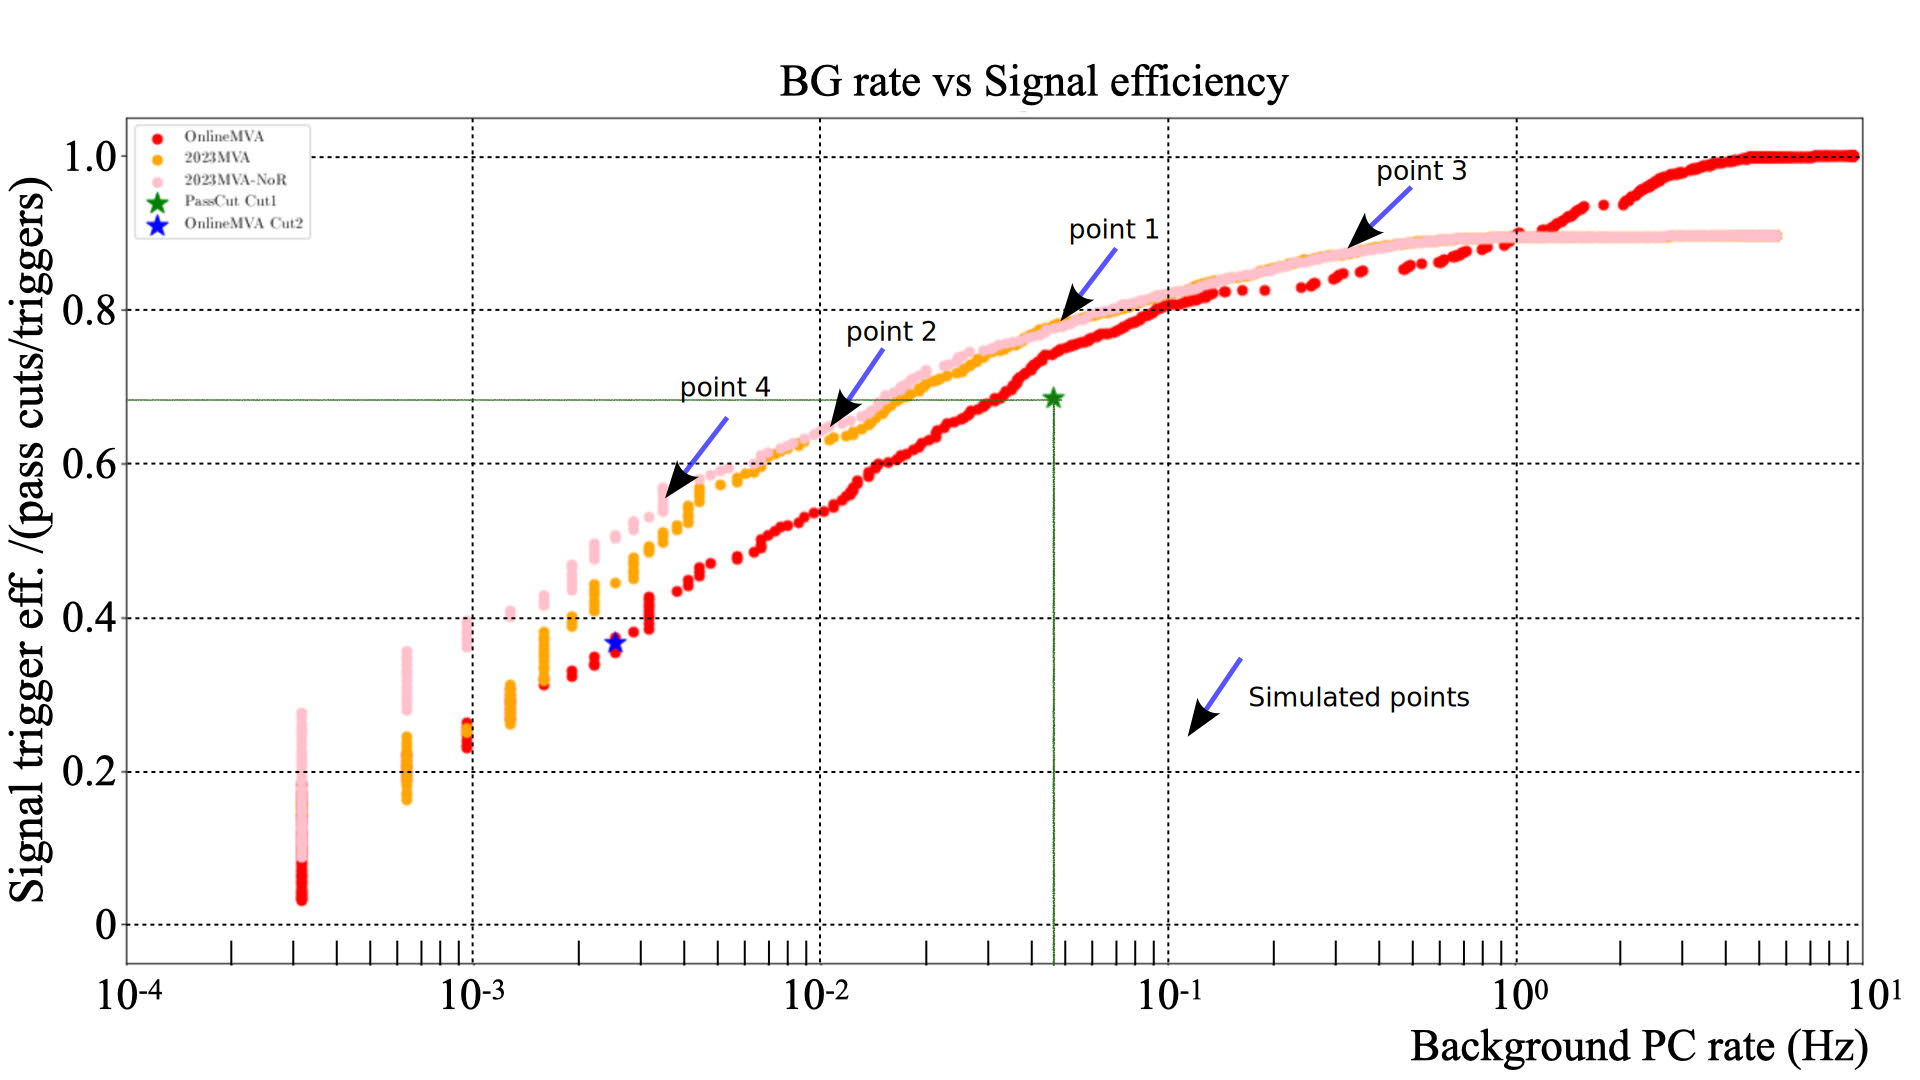
\includegraphics[width = \textwidth]{MVA.pdf}
\caption{MVA working curve.}
\end{figure}

\end{frame}


\begin{frame}{Results for \textit{Pass Cut} simulated data}

\begin{table}
\center
\resizebox{\textwidth}{!}{
\begin{tabular}{l|l l l l l}
\hline 
algorithms & $\mu$ $[\SI{}{\kilo \hertz}]$  
		   & $\sigma$  $[\SI{}{\kilo \hertz}]$
		   & $\mu$ $[\SI{}{\kilo \hertz}]$
		   & $\sigma$ $[\SI{}{\kilo \hertz}]$ \\ 
\hline
\textit{PassCut} data 						 	  &  \multicolumn{2}{c}{\color{blue}{without cosmic background}}     & \multicolumn{3}{c}{\color{blue}{with cosmic background}}  \\
\hline
2017 ($ > 0 ; > 1$ )          & $-0.18$  & $9.7$   & $-0.445$ & $14.1$\\ 

2017 reversed ($ < 3; < 2$)   & $+0.13$ & $7.89$   & $+0.25$  & $9.73$\\ 

threshold ($ > 1$)            & $+0.025$ & $11.5$  & $+0.005$ & $16.72$\\ 

threshold ($ > 2$)            & $-0.06$  & $9.56$  & $+0.67$  & $14.1$\\ 

threshold ($ > 3$)            & $-0.1$   & $7.48$  & $-0.07$  & $9.96$ \\

const. fraction ($ p = 10 \% $) & $-0.02$  & $11.56$ & $+0.19$   & $16.66$\\ 
 
const. fraction ($ p = 20 \% $) & $-0.215$ & $9.05$  & $+0.55$   & $13.06$\\ 

const. fraction ($ p = 30 \% $) & $+0.08$  & $7.43$  & $+0.05$   & $8.84$ \\

sumNeighbors ($ N = 1 $) & $+0.01$  & $9.47$  & $+0.055$   & $13.03$ \\

sumNeighbors ($ N = 2 $) & $-0.425$  & $8.83$  & $+0.005$   & $12.69$ \\

sumNeighbors ($ N = 3 $) & $-0.47$  & $7.85$  & $+0.115$   & $11.66$ \\
\hline
\end{tabular}}
\caption{ Result of the simulation for $N_{trials} = 1000$. In the first two column the cosmic background is removed from the data. The last two columns contains the result of the simulation adding the cosmic background. The $\mu$ and $\sigma$ are the quantities computed from the distribution of $(onset_{2} - onset_{1}) - MC_{truth}$.}
\end{table}
\end{frame}

\begin{frame}{Results for point 1 :$rate_{cosmic} = \SI{0.046}{\second \tothe{-1}}$, $\epsilon = 0.775$}

\begin{table}
\center
\resizebox{\textwidth}{!}{
\begin{tabular}{l|l l l l l}
\hline 
algorithms & $\mu$ $[\SI{}{\kilo \hertz}]$  
		   & $\sigma$  $[\SI{}{\kilo \hertz}]$
		   & $\mu$ $[\SI{}{\kilo \hertz}]$
		   & $\sigma$ $[\SI{}{\kilo \hertz}]$ \\ 
\hline
\textit{Point 1} data 						 	  &  \multicolumn{2}{c}{\color{blue}{without cosmic background}}     & \multicolumn{3}{c}{\color{blue}{with cosmic background}}  \\
\hline
2017 ($ > 0 ; > 1$ )          & $-0.045$  & $9.97$   & $-0.03$ & $13.68$\\ 

2017 reversed ($ < 3; < 2$)   & $-0.01$ & $8.15$   & $-0.3$  & $9.905$\\ 

threshold ($ > 1$)            & $+0.44$ & $11.37$  & $+0.54$ & $14.99$\\ 

threshold ($ > 2$)            & $+0.95$  & $9.96$  & $+0.39$  & $13.00$\\ 

threshold ($ > 3$)            & $+0.23$   & $7.50$  & $-0.17$  & $10.26$ \\

const. fraction ($ p = 10 \% $) & $+0.245$  & $11.71$ & $+0.745$   & $15.57$\\ 
 
const. fraction ($ p = 20 \% $) & $-0.115$ & $8.559$  & $+0.13$   & $11.1$\\ 

const. fraction ($ p = 30 \% $) & $+0.04$  & $6.79$  & $+0.085$   & $7.58$ \\

sumNeighbors ($ N = 1 $) & $+0.535$  & $9.303$  & $+0.25$   & $12.14$ \\

sumNeighbors ($ N = 2 $) & $+0.42$  & $8.915$  & $+0.195$   & $11.89$ \\

sumNeighbors ($ N = 3 $) & $+0.37$  & $8.177$  & $+0.175$   & $10.86$ \\
\hline
\end{tabular}}
\caption{ Result of the simulation for $N_{trials} = 1000$. In the first two column the cosmic background is removed from the data. The last two columns contains the result of the simulation adding the cosmic background. The $\mu$ and $\sigma$ are the quantities computed from the distribution of $(onset_{2} - onset_{1}) - MC_{truth}$.}
\end{table}
\end{frame}


\begin{frame}{Results for point 2 :$rate_{cosmic} = \SI{0.01}{\second \tothe{-1}}$, $\epsilon = 0.638$}

\begin{table}
\center
\resizebox{\textwidth}{!}{
\begin{tabular}{l|l l l l l}
\hline 
algorithms & $\mu$ $[\SI{}{\kilo \hertz}]$  
		   & $\sigma$  $[\SI{}{\kilo \hertz}]$
		   & $\mu$ $[\SI{}{\kilo \hertz}]$
		   & $\sigma$ $[\SI{}{\kilo \hertz}]$ \\ 
\hline
\textit{Point 2} data 						 	  &  \multicolumn{2}{c}{\color{blue}{without cosmic background}}     & \multicolumn{3}{c}{\color{blue}{with cosmic background}}  \\
\hline
2017 ($ > 0 ; > 1$ )          & $-0.35$  & $11.21$   & $-0.35$ & $11.21$\\ 

2017 reversed ($ < 3; < 2$)   & $+0.03$ & $8.19$   & $+0.03$  & $8.196$\\ 

threshold ($ > 1$)            & $-0.26$ & $12.69$  & $-0.26$ & $12.69$\\ 

threshold ($ > 2$)            & $-0.05$  & $10.28$  & $-0.05$  & $10.28$\\ 

threshold ($ > 3$)            & $+0.155$   & $7.93$  & $+0.155$  & $7.93$ \\

const. fraction ($ p = 10 \% $) & $-0.365$  & $12.75$ & $-0.365$   & $12.75$\\ 
 
const. fraction ($ p = 20 \% $) & $-0.005$ & $9.74$  & $-0.005$   & $9.74$\\ 

const. fraction ($ p = 30 \% $) & $+0.075$  & $7.725$  & $+0.075$   & $7.725$ \\

sumNeighbors ($ N = 1 $) & $-0.04$  & $10.67$  & $-0.04$   & $10.67$ \\

sumNeighbors ($ N = 2 $) & $-0.015$  & $11.06$  & $-0.015$   & $11.06$ \\

sumNeighbors ($ N = 3 $) & $-0.015$  & $11.06$  & $-0.015$   & $11.06$ \\
\hline
\end{tabular}}
\caption{ Result of the simulation for $N_{trials} = 1000$. In the first two column the cosmic background is removed from the data. The last two columns contains the result of the simulation adding the cosmic background. The $\mu$ and $\sigma$ are the quantities computed from the distribution of $(onset_{2} - onset_{1}) - MC_{truth}$.}
\end{table}
\end{frame}

\begin{frame}{Results for point 3 :$rate_{cosmic} = \SI{0.23}{\second \tothe{-1}}$, $\epsilon = 0.86$}

\begin{table}
\center
\resizebox{\textwidth}{!}{
\begin{tabular}{l|l l l l l}
\hline 
algorithms & $\mu$ $[\SI{}{\kilo \hertz}]$  
		   & $\sigma$  $[\SI{}{\kilo \hertz}]$
		   & $\mu$ $[\SI{}{\kilo \hertz}]$
		   & $\sigma$ $[\SI{}{\kilo \hertz}]$ \\ 
\hline
\textit{Point 3} data 						 	  &  \multicolumn{2}{c}{\color{blue}{without cosmic background}}     & \multicolumn{3}{c}{\color{blue}{with cosmic background}}  \\
\hline
2017 ($ > 0 ; > 1$ )          & $-0.04$  & \textcolor{red}{$10.47$*}   & $+0.31$ & \textcolor{red}{$10.2$*}\\ 

2017 reversed ($ < 3; < 2$)   & $+0.15$ & $8.51$   & $-0.7731$  & $13.45$\\ 

threshold ($ > 1$)            & $+0.295$ & \textcolor{red}{$11.18$*}  & $-0.24$ & \textcolor{red}{$8.06$*}\\ 

threshold ($ > 2$)            & $+0.42$  & $10.08$  & $+0.16$  & $13.92$\\ 

threshold ($ > 3$)            & $+0.455$   & $8.026$  & $+0.165$  & $18.73$ \\

const. fraction ($ p = 10 \% $) & $+0.18$  & $11.81$ & $+0.125$   & $13.19$\\ 
 
const. fraction ($ p = 20 \% $) & $+0.08$ & $8.23$  & $-1.12$   & $20.4$\\ 

const. fraction ($ p = 30 \% $) & $-0.185$  & $6.26$  & $-0.125$   & $14.59$ \\

sumNeighbors ($ N = 1 $) & $+0.005$  & $6.00$  & $+0.19$   & $14.75$ \\

sumNeighbors ($ N = 2 $) & $-0.115$  & $4.77$  & $+0.265$   & $13.39$ \\

sumNeighbors ($ N = 3 $) & $-0.1$  & $4.43$  & $-0.31$   & $10.16$ \\
\hline
\end{tabular}}
\caption{ Result of the simulation for $N_{trials} = 1000$. In the first two column the cosmic background is removed from the data. The last two columns contains the result of the simulation adding the cosmic background. The $\mu$ and $\sigma$ are the quantities computed from the distribution of $(onset_{2} - onset_{1}) - MC_{truth}$.}
\end{table}

\textcolor{red}{*} These values shows an unpredicted behaviour: $\sigma$ with cosmic background is lower compared to the $\sigma$ without cosmic background. Looking at figure \ref{fig:HighCosmicError} we observe that the high cosmic rate "triggers" the algorithms, which identifies systematically the initial frequency of the sweep as onset. Consequently, the result are significantly affected by this unwanted behaviour.    

\end{frame}

\begin{frame}

\begin{figure}[hbtp]
\centering
\includegraphics[width = \textwidth]{../LineShape/Plot/point3/Threshold_1.pdf}
\caption{Result for algorithm \textit{Threshold ($> 1$)} with cosmic background. Due to the high cosmic rate, the algorithm identifies sistematically the first bin of the sweep. This reduces artificially the $\sigma$ of the $(onset_{2} - onset_{1}) - MC_{truth}$, however this is an unintended behaviour, and we plan to fix it.}
\label{fig:HighCosmicError}
\end{figure}


\end{frame}


\begin{frame}{ \textit{PassCut} plots}

\begin{figure}
\centering
\subfloat[][\emph{algorithm 2017}]
{\includegraphics[width=.30\textwidth]{../LineShape/Plot/delta_2017_foward.pdf}} 
\subfloat[][\emph{algorithm 2017 reversed}]
{\includegraphics[width=.30\textwidth]{../LineShape/Plot/delta_2017_reversed.pdf}} 
\subfloat[][\emph{threshold ($> 2$)}]
{\includegraphics[width=.30\textwidth]{../LineShape/Plot/delta_Threshold_2.pdf}} \\
\subfloat[][\emph{threshold ($> 3$)}]
{\includegraphics[width=.30\textwidth]{../LineShape/Plot/delta_Threshold_3.pdf}}
\subfloat[][\emph{const fraction ($> 20\%$)}]
{\includegraphics[width=.30\textwidth]{../LineShape/Plot/delta_constFract_20.pdf}} 
\subfloat[][\emph{const fraction ($> 30\%$)}]
{\includegraphics[width=.30\textwidth]{../LineShape/Plot/delta_constFract_30.pdf}}
\end{figure}
\end{frame}

\begin{frame}{ \textit{PassCut} plots}

\begin{figure}
\centering
\subfloat[][\emph{sumNeighbors ($N > 2$)}]
{\includegraphics[width=.45\textwidth]{../LineShape/Plot/delta_sumNeighbors_sigma20.pdf}}
\subfloat[][\emph{sumNeighbors ($N > 3$)}]
{\includegraphics[width=.45\textwidth]{../LineShape/Plot/delta_sumNeighbors_sigma30.pdf}}
\end{figure}
\end{frame}


\begin{frame}{Next steps}

\begin{itemize}
\item Add to the simulation the magnetic field drift
\item Systematic studies of the relative shape asymmetry for the two transitions and its effect on the onset determination.
\end{itemize}
\end{frame}

\end{document}